% Options for packages loaded elsewhere
\PassOptionsToPackage{unicode}{hyperref}
\PassOptionsToPackage{hyphens}{url}
%
\documentclass[
]{article}
\usepackage{lmodern}
\usepackage{amssymb,amsmath}
\usepackage{ifxetex,ifluatex}
\ifnum 0\ifxetex 1\fi\ifluatex 1\fi=0 % if pdftex
  \usepackage[T1]{fontenc}
  \usepackage[utf8]{inputenc}
  \usepackage{textcomp} % provide euro and other symbols
\else % if luatex or xetex
  \usepackage{unicode-math}
  \defaultfontfeatures{Scale=MatchLowercase}
  \defaultfontfeatures[\rmfamily]{Ligatures=TeX,Scale=1}
\fi
% Use upquote if available, for straight quotes in verbatim environments
\IfFileExists{upquote.sty}{\usepackage{upquote}}{}
\IfFileExists{microtype.sty}{% use microtype if available
  \usepackage[]{microtype}
  \UseMicrotypeSet[protrusion]{basicmath} % disable protrusion for tt fonts
}{}
\makeatletter
\@ifundefined{KOMAClassName}{% if non-KOMA class
  \IfFileExists{parskip.sty}{%
    \usepackage{parskip}
  }{% else
    \setlength{\parindent}{0pt}
    \setlength{\parskip}{6pt plus 2pt minus 1pt}}
}{% if KOMA class
  \KOMAoptions{parskip=half}}
\makeatother
\usepackage{xcolor}
\IfFileExists{xurl.sty}{\usepackage{xurl}}{} % add URL line breaks if available
\IfFileExists{bookmark.sty}{\usepackage{bookmark}}{\usepackage{hyperref}}
\hypersetup{
  pdftitle={Stochastic Processes: Assignment 1},
  pdfauthor={Javier Esteban Aragoneses, Mauricio Marcos Fajgenbaun, Danyu Zhang, Daniel Alonso},
  hidelinks,
  pdfcreator={LaTeX via pandoc}}
\urlstyle{same} % disable monospaced font for URLs
\usepackage[margin=1in]{geometry}
\usepackage{color}
\usepackage{fancyvrb}
\newcommand{\VerbBar}{|}
\newcommand{\VERB}{\Verb[commandchars=\\\{\}]}
\DefineVerbatimEnvironment{Highlighting}{Verbatim}{commandchars=\\\{\}}
% Add ',fontsize=\small' for more characters per line
\usepackage{framed}
\definecolor{shadecolor}{RGB}{248,248,248}
\newenvironment{Shaded}{\begin{snugshade}}{\end{snugshade}}
\newcommand{\AlertTok}[1]{\textcolor[rgb]{0.94,0.16,0.16}{#1}}
\newcommand{\AnnotationTok}[1]{\textcolor[rgb]{0.56,0.35,0.01}{\textbf{\textit{#1}}}}
\newcommand{\AttributeTok}[1]{\textcolor[rgb]{0.77,0.63,0.00}{#1}}
\newcommand{\BaseNTok}[1]{\textcolor[rgb]{0.00,0.00,0.81}{#1}}
\newcommand{\BuiltInTok}[1]{#1}
\newcommand{\CharTok}[1]{\textcolor[rgb]{0.31,0.60,0.02}{#1}}
\newcommand{\CommentTok}[1]{\textcolor[rgb]{0.56,0.35,0.01}{\textit{#1}}}
\newcommand{\CommentVarTok}[1]{\textcolor[rgb]{0.56,0.35,0.01}{\textbf{\textit{#1}}}}
\newcommand{\ConstantTok}[1]{\textcolor[rgb]{0.00,0.00,0.00}{#1}}
\newcommand{\ControlFlowTok}[1]{\textcolor[rgb]{0.13,0.29,0.53}{\textbf{#1}}}
\newcommand{\DataTypeTok}[1]{\textcolor[rgb]{0.13,0.29,0.53}{#1}}
\newcommand{\DecValTok}[1]{\textcolor[rgb]{0.00,0.00,0.81}{#1}}
\newcommand{\DocumentationTok}[1]{\textcolor[rgb]{0.56,0.35,0.01}{\textbf{\textit{#1}}}}
\newcommand{\ErrorTok}[1]{\textcolor[rgb]{0.64,0.00,0.00}{\textbf{#1}}}
\newcommand{\ExtensionTok}[1]{#1}
\newcommand{\FloatTok}[1]{\textcolor[rgb]{0.00,0.00,0.81}{#1}}
\newcommand{\FunctionTok}[1]{\textcolor[rgb]{0.00,0.00,0.00}{#1}}
\newcommand{\ImportTok}[1]{#1}
\newcommand{\InformationTok}[1]{\textcolor[rgb]{0.56,0.35,0.01}{\textbf{\textit{#1}}}}
\newcommand{\KeywordTok}[1]{\textcolor[rgb]{0.13,0.29,0.53}{\textbf{#1}}}
\newcommand{\NormalTok}[1]{#1}
\newcommand{\OperatorTok}[1]{\textcolor[rgb]{0.81,0.36,0.00}{\textbf{#1}}}
\newcommand{\OtherTok}[1]{\textcolor[rgb]{0.56,0.35,0.01}{#1}}
\newcommand{\PreprocessorTok}[1]{\textcolor[rgb]{0.56,0.35,0.01}{\textit{#1}}}
\newcommand{\RegionMarkerTok}[1]{#1}
\newcommand{\SpecialCharTok}[1]{\textcolor[rgb]{0.00,0.00,0.00}{#1}}
\newcommand{\SpecialStringTok}[1]{\textcolor[rgb]{0.31,0.60,0.02}{#1}}
\newcommand{\StringTok}[1]{\textcolor[rgb]{0.31,0.60,0.02}{#1}}
\newcommand{\VariableTok}[1]{\textcolor[rgb]{0.00,0.00,0.00}{#1}}
\newcommand{\VerbatimStringTok}[1]{\textcolor[rgb]{0.31,0.60,0.02}{#1}}
\newcommand{\WarningTok}[1]{\textcolor[rgb]{0.56,0.35,0.01}{\textbf{\textit{#1}}}}
\usepackage{graphicx}
\makeatletter
\def\maxwidth{\ifdim\Gin@nat@width>\linewidth\linewidth\else\Gin@nat@width\fi}
\def\maxheight{\ifdim\Gin@nat@height>\textheight\textheight\else\Gin@nat@height\fi}
\makeatother
% Scale images if necessary, so that they will not overflow the page
% margins by default, and it is still possible to overwrite the defaults
% using explicit options in \includegraphics[width, height, ...]{}
\setkeys{Gin}{width=\maxwidth,height=\maxheight,keepaspectratio}
% Set default figure placement to htbp
\makeatletter
\def\fps@figure{htbp}
\makeatother
\setlength{\emergencystretch}{3em} % prevent overfull lines
\providecommand{\tightlist}{%
  \setlength{\itemsep}{0pt}\setlength{\parskip}{0pt}}
\setcounter{secnumdepth}{-\maxdimen} % remove section numbering
\ifluatex
  \usepackage{selnolig}  % disable illegal ligatures
\fi

\title{Stochastic Processes: Assignment 1}
\author{Javier Esteban Aragoneses, Mauricio Marcos Fajgenbaun, Danyu
Zhang, Daniel Alonso}
\date{November 27th, 2020}

\begin{document}
\maketitle

Importing libraries

\begin{Shaded}
\begin{Highlighting}[]
\FunctionTok{library}\NormalTok{(markovchain)}
\FunctionTok{library}\NormalTok{(matlib)}
\end{Highlighting}
\end{Shaded}

Function to solve the problems

\begin{Shaded}
\begin{Highlighting}[]
\CommentTok{\# Thanks profe!}
\NormalTok{matrixpower }\OtherTok{\textless{}{-}} \ControlFlowTok{function}\NormalTok{(M,k) \{}
  \ControlFlowTok{if}\NormalTok{(}\FunctionTok{dim}\NormalTok{(M)[}\DecValTok{1}\NormalTok{]}\SpecialCharTok{!=}\FunctionTok{dim}\NormalTok{(M)[}\DecValTok{2}\NormalTok{]) }\FunctionTok{return}\NormalTok{(}\FunctionTok{print}\NormalTok{(}\StringTok{"Error: matrix M is not square"}\NormalTok{))}
  \ControlFlowTok{if}\NormalTok{ (k }\SpecialCharTok{==} \DecValTok{0}\NormalTok{) }\FunctionTok{return}\NormalTok{(}\FunctionTok{diag}\NormalTok{(}\FunctionTok{dim}\NormalTok{(M)[}\DecValTok{1}\NormalTok{])) }
  \ControlFlowTok{if}\NormalTok{ (k }\SpecialCharTok{==} \DecValTok{1}\NormalTok{) }\FunctionTok{return}\NormalTok{(M)}
  \ControlFlowTok{if}\NormalTok{ (k }\SpecialCharTok{\textgreater{}} \DecValTok{1}\NormalTok{)  }\FunctionTok{return}\NormalTok{(M }\SpecialCharTok{\%*\%} \FunctionTok{matrixpower}\NormalTok{(M, k}\DecValTok{{-}1}\NormalTok{))}
\NormalTok{\}}
\end{Highlighting}
\end{Shaded}

\hypertarget{problem-1}{%
\section{Problem 1}\label{problem-1}}

\hypertarget{a}{%
\subsection{a)}\label{a}}

Markov chain criteria:

1- The probability of being in a state only depends on the previous
state.

2- It's a stochastic process.

\(X\) = The chain hits state \(j\) at time \(n\)

\(X_{n}\) is the scenario at time \(n\)

All states have finite expected return times and there is only a single
communication class so the MC is irreducible, therefore its stationary
distribution is \textbf{unique}.

\begin{figure}
\centering
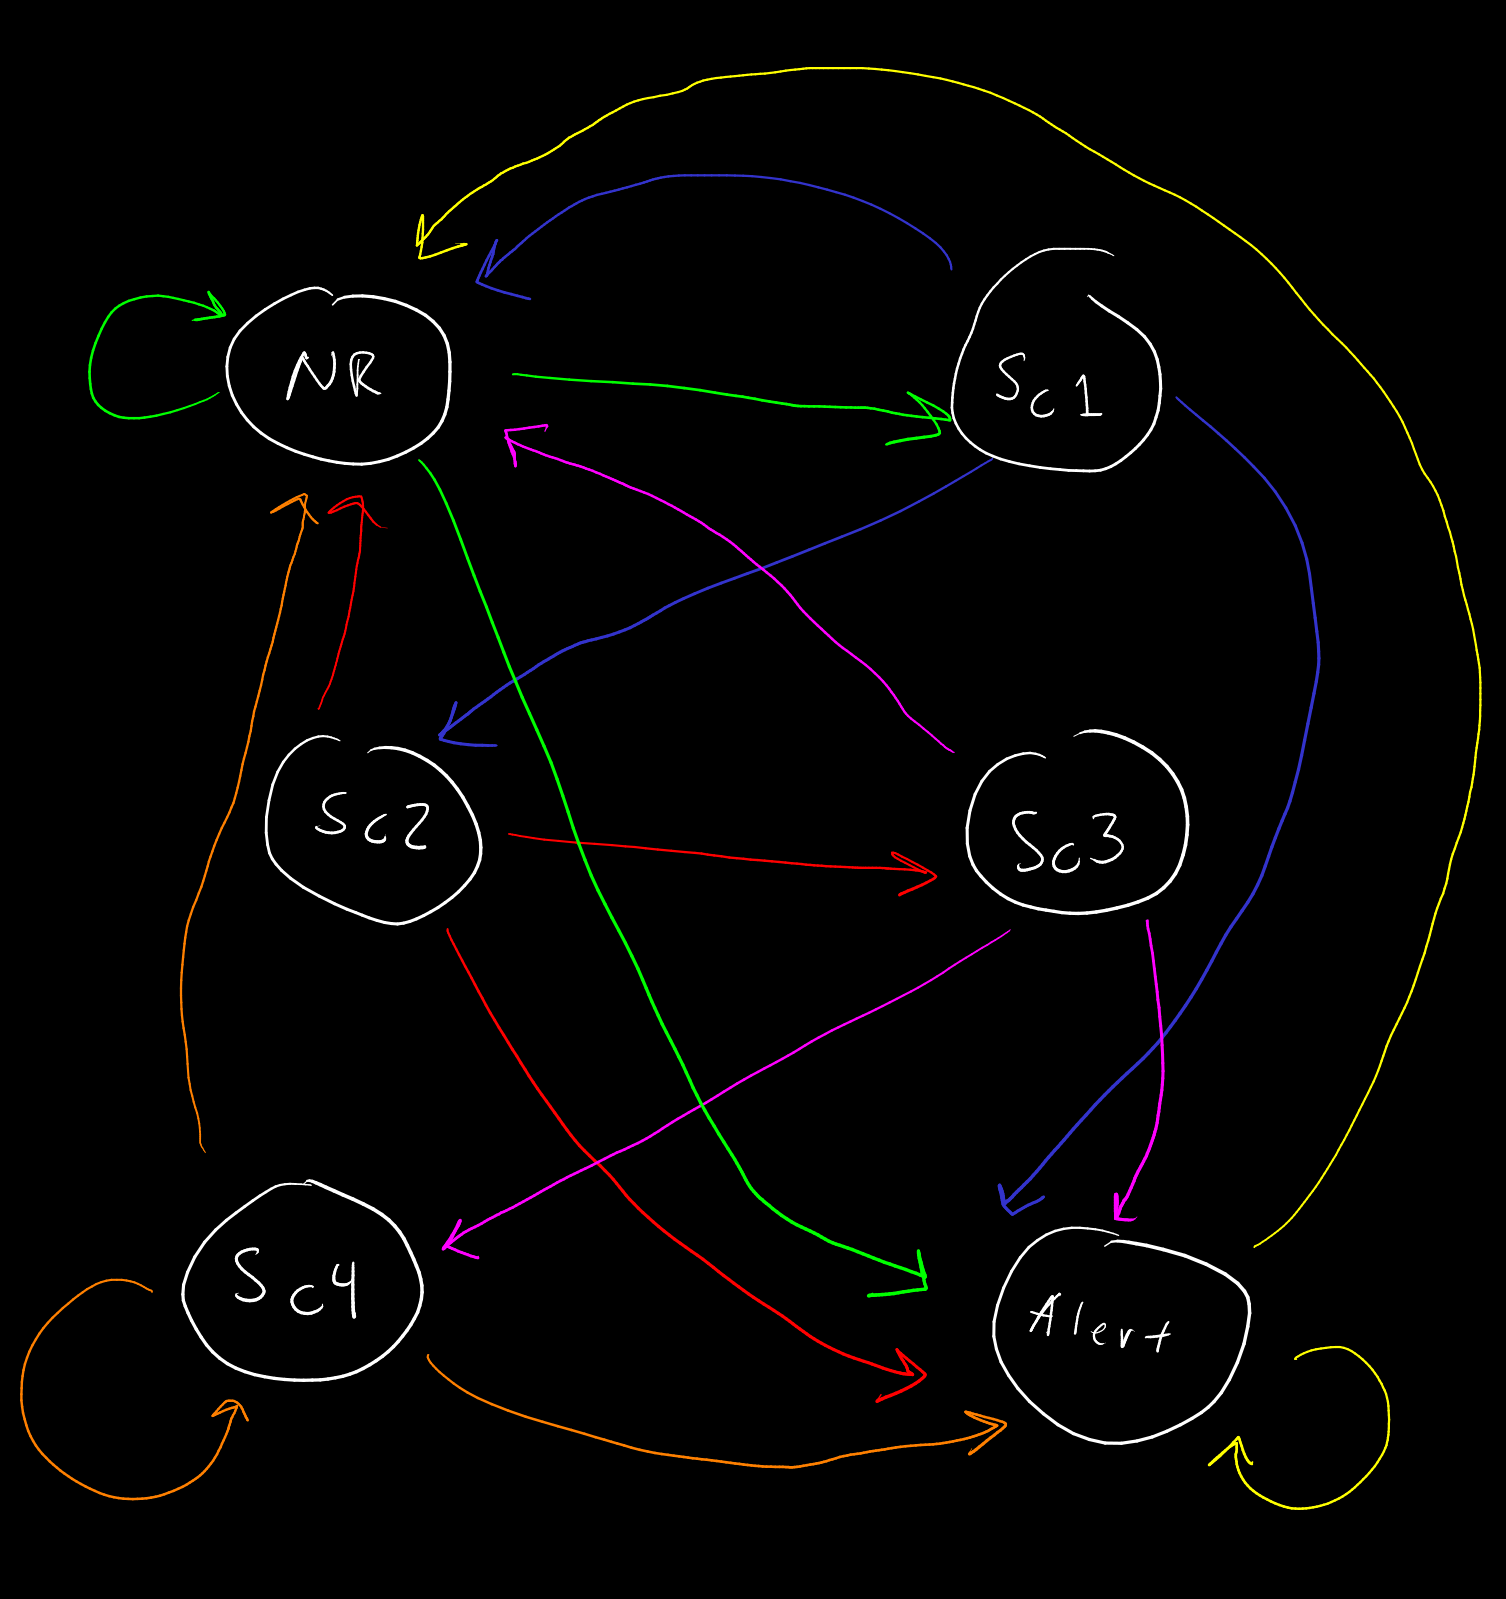
\includegraphics{./grafo1.png}
\caption{Graph for prob.1}
\end{figure}

\newpage

\hypertarget{b}{%
\subsection{b)}\label{b}}

We have first calculated the relative frequencies manually.

\begin{Shaded}
\begin{Highlighting}[]
\FunctionTok{load}\NormalTok{(}\StringTok{\textquotesingle{}PollutionMadrid.RData\textquotesingle{}}\NormalTok{)}
\NormalTok{data }\OtherTok{\textless{}{-}}\NormalTok{  X[}\DecValTok{1}\NormalTok{,]}
\NormalTok{mat }\OtherTok{\textless{}{-}} \FunctionTok{matrix}\NormalTok{(}\FunctionTok{rep}\NormalTok{(}\DecValTok{0}\NormalTok{,}\DecValTok{36}\NormalTok{), }\AttributeTok{nrow=}\DecValTok{6}\NormalTok{, }\AttributeTok{byrow=}\NormalTok{T)}
\ControlFlowTok{for}\NormalTok{ (i }\ControlFlowTok{in} \DecValTok{1}\SpecialCharTok{:}\FunctionTok{length}\NormalTok{(data)) \{}
  \ControlFlowTok{if}\NormalTok{ (data[i] }\SpecialCharTok{==} \StringTok{"Alert"}\NormalTok{) \{}
\NormalTok{    data[i] }\OtherTok{=} \DecValTok{1}
\NormalTok{  \} }\ControlFlowTok{else} \ControlFlowTok{if}\NormalTok{ (data[i] }\SpecialCharTok{==} \StringTok{"NR"}\NormalTok{) \{}
\NormalTok{    data[i] }\OtherTok{=} \DecValTok{2}
\NormalTok{  \} }\ControlFlowTok{else} \ControlFlowTok{if}\NormalTok{ (data[i] }\SpecialCharTok{==} \StringTok{"Sc1"}\NormalTok{) \{}
\NormalTok{    data[i] }\OtherTok{=} \DecValTok{3}
\NormalTok{  \} }\ControlFlowTok{else} \ControlFlowTok{if}\NormalTok{ (data[i] }\SpecialCharTok{==} \StringTok{"Sc2"}\NormalTok{) \{}
\NormalTok{    data[i] }\OtherTok{=} \DecValTok{4} 
\NormalTok{  \} }\ControlFlowTok{else} \ControlFlowTok{if}\NormalTok{ (data[i] }\SpecialCharTok{==} \StringTok{"Sc3"}\NormalTok{) \{}
\NormalTok{    data[i] }\OtherTok{=} \DecValTok{5}
\NormalTok{  \} }\ControlFlowTok{else} \ControlFlowTok{if}\NormalTok{ (data[i] }\SpecialCharTok{==} \StringTok{"Sc4"}\NormalTok{) \{}
\NormalTok{    data[i] }\OtherTok{=} \DecValTok{6}
\NormalTok{  \}}
\NormalTok{\}}
\NormalTok{data }\OtherTok{\textless{}{-}} \FunctionTok{as.numeric}\NormalTok{(data)}
\ControlFlowTok{for}\NormalTok{ (i }\ControlFlowTok{in} \DecValTok{1}\SpecialCharTok{:}\FunctionTok{length}\NormalTok{(data)) \{}
\NormalTok{  mat[data[i],data[i}\SpecialCharTok{+}\DecValTok{1}\NormalTok{]] }\OtherTok{=}\NormalTok{ mat[data[i],data[i}\SpecialCharTok{+}\DecValTok{1}\NormalTok{]] }\SpecialCharTok{+} \DecValTok{1}
\NormalTok{\}}
\NormalTok{mat[data[}\DecValTok{1460}\NormalTok{],data[}\DecValTok{1}\NormalTok{]] }\OtherTok{=}\NormalTok{ mat[data[}\DecValTok{1460}\NormalTok{],data[}\DecValTok{1}\NormalTok{]] }\SpecialCharTok{+} \DecValTok{1}

\NormalTok{tbl }\OtherTok{\textless{}{-}} \FunctionTok{table}\NormalTok{(data)}
\ControlFlowTok{for}\NormalTok{ (i }\ControlFlowTok{in} \DecValTok{1}\SpecialCharTok{:}\FunctionTok{length}\NormalTok{(tbl)) \{}
\NormalTok{  mat[i,] }\OtherTok{=}\NormalTok{ mat[i,]}\SpecialCharTok{/}\NormalTok{tbl[i]}
\NormalTok{\}}
\NormalTok{mat}
\CommentTok{\#\textgreater{}            [,1]      [,2]       [,3]      [,4]      [,5]      [,6]}
\CommentTok{\#\textgreater{} [1,] 0.00000000 1.0000000 0.00000000 0.0000000 0.0000000 0.0000000}
\CommentTok{\#\textgreater{} [2,] 0.00000000 0.9529851 0.04701493 0.0000000 0.0000000 0.0000000}
\CommentTok{\#\textgreater{} [3,] 0.01587302 0.4920635 0.00000000 0.4920635 0.0000000 0.0000000}
\CommentTok{\#\textgreater{} [4,] 0.00000000 0.5806452 0.00000000 0.0000000 0.4193548 0.0000000}
\CommentTok{\#\textgreater{} [5,] 0.23076923 0.3846154 0.00000000 0.0000000 0.0000000 0.3846154}
\CommentTok{\#\textgreater{} [6,] 0.00000000 0.5555556 0.00000000 0.0000000 0.0000000 0.4444444}
\end{Highlighting}
\end{Shaded}

\newpage

We then tested using the \emph{markovchain} package in order to confirm
our results.

\begin{Shaded}
\begin{Highlighting}[]
\NormalTok{data }\OtherTok{\textless{}{-}}\NormalTok{ X[}\DecValTok{1}\NormalTok{,]}
\FunctionTok{markovchainFit}\NormalTok{(data)}\SpecialCharTok{$}\NormalTok{estimate}
\CommentTok{\#\textgreater{} MLE Fit }
\CommentTok{\#\textgreater{}  A  6 {-} dimensional discrete Markov Chain defined by the following states: }
\CommentTok{\#\textgreater{}  Alert, NR, Sc1, Sc2, Sc3, Sc4 }
\CommentTok{\#\textgreater{}  The transition matrix  (by rows)  is defined as follows: }
\CommentTok{\#\textgreater{}            Alert        NR        Sc1 Sc2       Sc3       Sc4}
\CommentTok{\#\textgreater{} Alert 0.00000000 1.0000000 0.00000000 0.0 0.0000000 0.0000000}
\CommentTok{\#\textgreater{} NR    0.00000000 0.9529851 0.04701493 0.0 0.0000000 0.0000000}
\CommentTok{\#\textgreater{} Sc1   0.01612903 0.4838710 0.00000000 0.5 0.0000000 0.0000000}
\CommentTok{\#\textgreater{} Sc2   0.00000000 0.5806452 0.00000000 0.0 0.4193548 0.0000000}
\CommentTok{\#\textgreater{} Sc3   0.23076923 0.3846154 0.00000000 0.0 0.0000000 0.3846154}
\CommentTok{\#\textgreater{} Sc4   0.00000000 0.5555556 0.00000000 0.0 0.0000000 0.4444444}
\end{Highlighting}
\end{Shaded}

~

\hypertarget{what-can-you-say-of-the-comparison-of-your-estimates-andthe-possible-transitions-between-states-that-you-had-argued-in-part-a}{%
\subsubsection{What can you say of the comparison of your estimates
andthe possible transitions between states that you had argued in part
a}\label{what-can-you-say-of-the-comparison-of-your-estimates-andthe-possible-transitions-between-states-that-you-had-argued-in-part-a}}

According to our probabilities shown in the graph. There are 3 arrows
with probability 0. This is due to the fact that in the data there are
zero transitions from \(Sc2 \rightarrow Alert\),
\(Sc4 \rightarrow Alert\), \(NR \rightarrow Alert\),
\(Alert \rightarrow Alert\).

This is logical given that it is very unlikely to hit an alert state.
Unlike the rest of the states.

Later it will be shown that there's a unique stationary distribution
(see 1d).

\begin{figure}
\centering
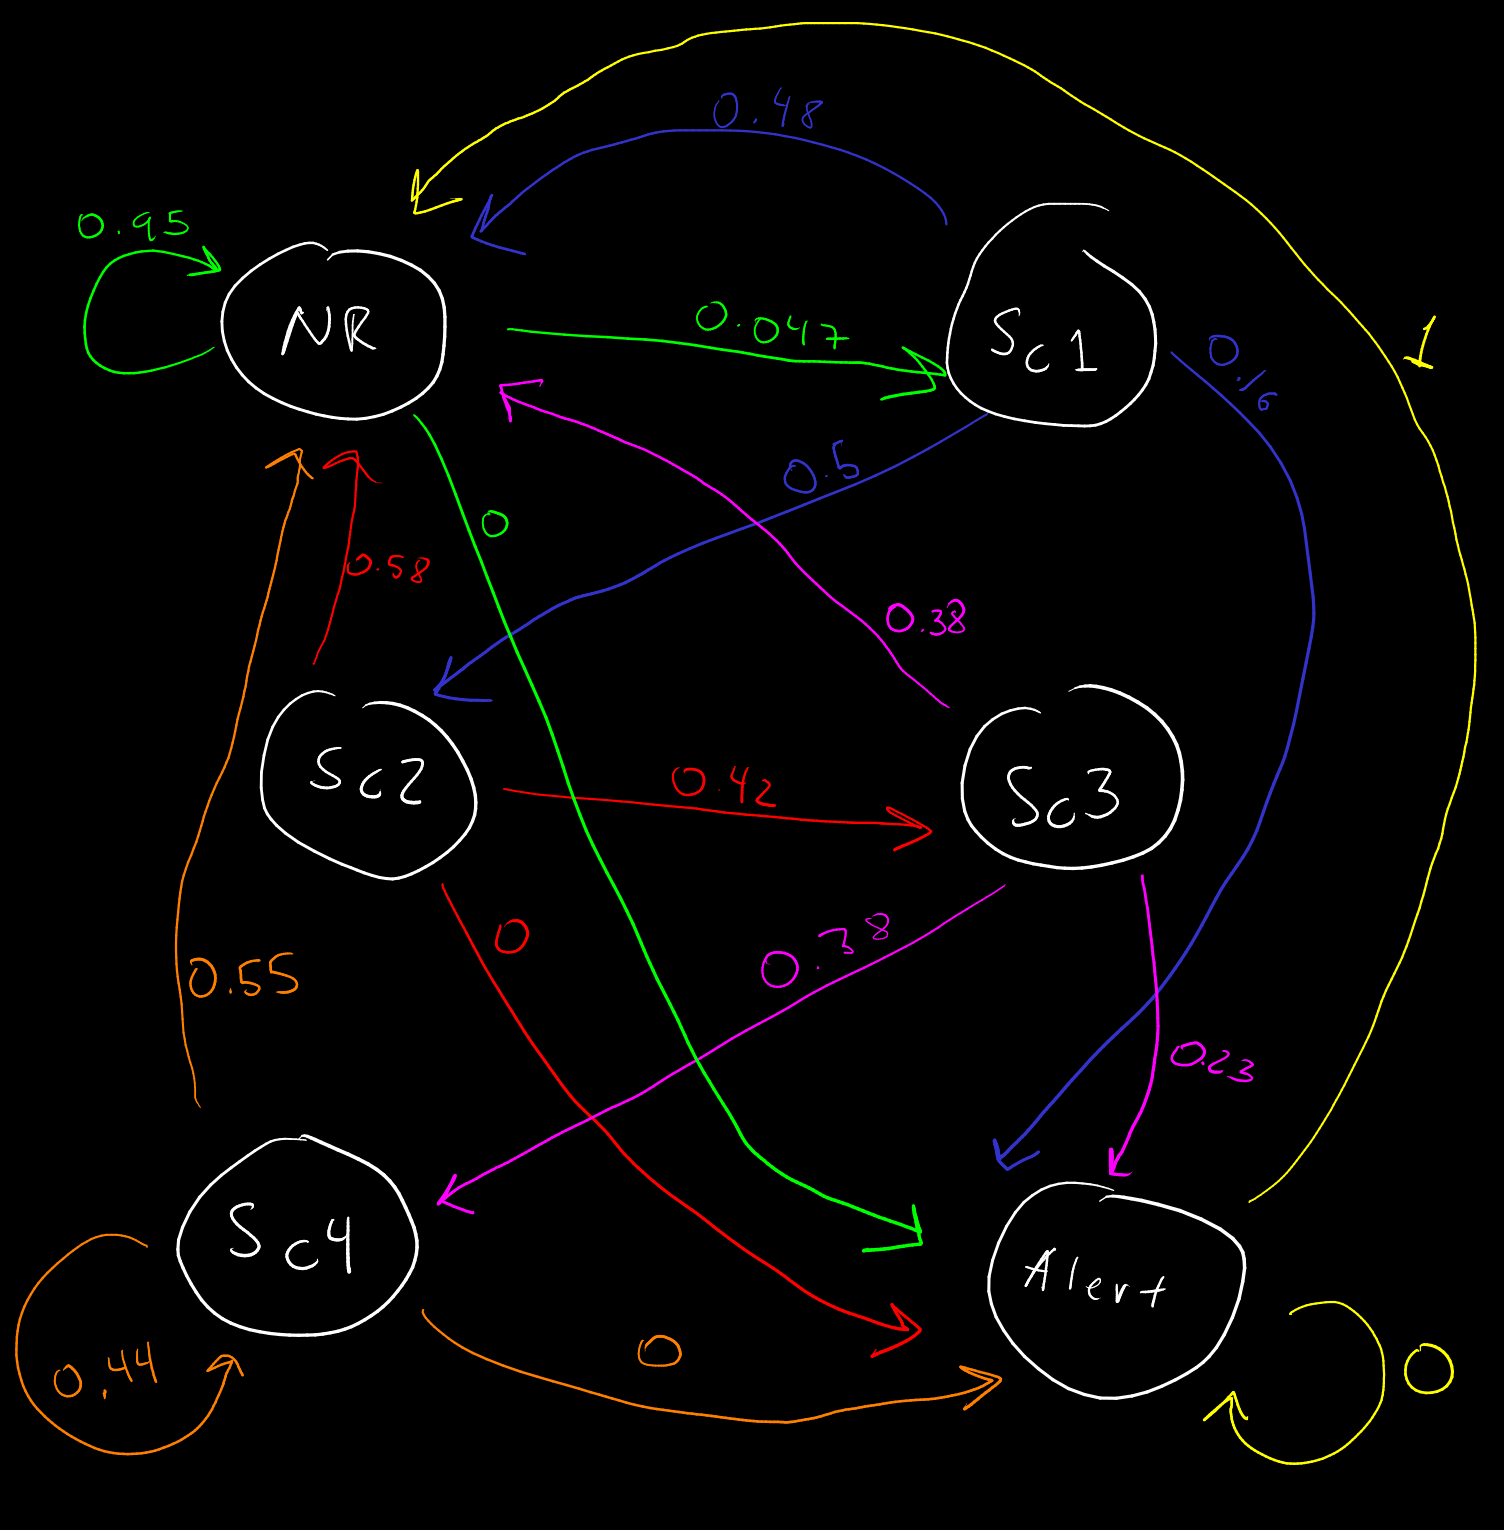
\includegraphics{./grafo1_probs.png}
\caption{Graph with probabilities for problem 1 (b)}
\end{figure}

\newpage

\hypertarget{c}{%
\subsection{c)}\label{c}}

Given that the first state of the chain is NR. We see the following 7
states:

\begin{Shaded}
\begin{Highlighting}[]
\NormalTok{data[}\DecValTok{1}\SpecialCharTok{:}\DecValTok{7}\NormalTok{]}
\CommentTok{\#\textgreater{} [1] "NR" "NR" "NR" "NR" "NR" "NR" "NR"}
\end{Highlighting}
\end{Shaded}

And we calculate the probability as follows:

\begin{Shaded}
\begin{Highlighting}[]
\NormalTok{mat[}\DecValTok{2}\NormalTok{,}\DecValTok{2}\NormalTok{]}\SpecialCharTok{\^{}}\DecValTok{7}
\CommentTok{\#\textgreater{} [1] 0.713843}
\end{Highlighting}
\end{Shaded}

We can see the probability is 0.713843

\hypertarget{d}{%
\subsection{d)}\label{d}}

We can see that because we have a unique solution to the system, we have
a unique stationary distribution.

\begin{Shaded}
\begin{Highlighting}[]
\NormalTok{stationary\_dist }\OtherTok{\textless{}{-}} \ControlFlowTok{function}\NormalTok{(P) \{}
\NormalTok{    dim }\OtherTok{=} \FunctionTok{sqrt}\NormalTok{(}\FunctionTok{length}\NormalTok{(P))}
\NormalTok{    A }\OtherTok{=}\NormalTok{ P }\SpecialCharTok{{-}} \FunctionTok{diag}\NormalTok{(dim)}
\NormalTok{    b }\OtherTok{=} \FunctionTok{matrix}\NormalTok{(}\FunctionTok{c}\NormalTok{(}\DecValTok{1}\NormalTok{,}\FunctionTok{rep}\NormalTok{(}\DecValTok{0}\NormalTok{,dim}\DecValTok{{-}1}\NormalTok{)),}\AttributeTok{nrow=}\NormalTok{dim,}\AttributeTok{byrow=}\NormalTok{T)}
\NormalTok{    A[,}\DecValTok{1}\NormalTok{] }\OtherTok{\textless{}{-}} \FunctionTok{rep}\NormalTok{(}\DecValTok{1}\NormalTok{,dim)}
    \FunctionTok{print}\NormalTok{(}\StringTok{"The solution is the following:"}\NormalTok{)}
    \FunctionTok{return}\NormalTok{(matlib}\SpecialCharTok{::}\FunctionTok{Solve}\NormalTok{(}\FunctionTok{t}\NormalTok{(A), b))}
\NormalTok{\}}
\NormalTok{stat\_dist }\OtherTok{\textless{}{-}} \FunctionTok{stationary\_dist}\NormalTok{(mat)}
\CommentTok{\#\textgreater{} [1] "The solution is the following:"}
\CommentTok{\#\textgreater{} x1            =  0.00273973 }
\CommentTok{\#\textgreater{}   x2          =  0.91780822 }
\CommentTok{\#\textgreater{}     x3        =  0.04315068 }
\CommentTok{\#\textgreater{}       x4      =  0.02123288 }
\CommentTok{\#\textgreater{}         x5    =  0.00890411 }
\CommentTok{\#\textgreater{}           x6  =  0.00616438}
\NormalTok{stat\_dist}
\CommentTok{\#\textgreater{} [1] "x1            =  0.00273973" "  x2          =  0.91780822"}
\CommentTok{\#\textgreater{} [3] "    x3        =  0.04315068" "      x4      =  0.02123288"}
\CommentTok{\#\textgreater{} [5] "        x5    =  0.00890411" "          x6  =  0.00616438"}
\end{Highlighting}
\end{Shaded}

This is our stationary distribution:

\(\pi_{1} = 0.00273973\)

\(\pi_{2} = 0.91780822\)

\(\pi_{3} = 0.04315068\)

\(\pi_{4} = 0.02123288\)

\(\pi_{5} = 0.00890411\)

\(\pi_{6} = 0.00616438\)

\newpage

Comparing with the proportions we get from our data:

\begin{Shaded}
\begin{Highlighting}[]
\NormalTok{rel\_error }\OtherTok{=} \FunctionTok{c}\NormalTok{()}
\NormalTok{props }\OtherTok{=} \FunctionTok{table}\NormalTok{(data)}\SpecialCharTok{/}\FunctionTok{length}\NormalTok{(data)}
\NormalTok{results }\OtherTok{\textless{}{-}} \FunctionTok{c}\NormalTok{(}\FloatTok{0.00273973}\NormalTok{,}\FloatTok{0.91780822}\NormalTok{,}\FloatTok{0.04315068}\NormalTok{,}\FloatTok{0.02123288}\NormalTok{,}\FloatTok{0.00890411}\NormalTok{,}\FloatTok{0.00616438}\NormalTok{)}
\ControlFlowTok{for}\NormalTok{ (i }\ControlFlowTok{in} \DecValTok{1}\SpecialCharTok{:}\FunctionTok{length}\NormalTok{(props)) \{}
\NormalTok{    rel\_error[i] }\OtherTok{\textless{}{-}} \FunctionTok{abs}\NormalTok{(props[i]}\SpecialCharTok{{-}}\NormalTok{results[i])}\SpecialCharTok{/}\NormalTok{results[i]}
\NormalTok{\}}
\NormalTok{rel\_error}
\CommentTok{\#\textgreater{} [1] 1.449998e{-}06 8.955223e{-}10 1.142857e{-}07 1.548387e{-}07 4.615384e{-}08}
\CommentTok{\#\textgreater{} [6] 5.777781e{-}07}
\end{Highlighting}
\end{Shaded}

We can see our relative errors are all quite low
(\textless{}\(1*10^{-5}\)) so we could say that the difference between
both estimations is nearly negligible.

\hypertarget{e}{%
\subsection{e)}\label{e}}

\hypertarget{proof-that-this-mc-has-a-limiting-distribution}{%
\subsubsection{Proof that this MC has a limiting
distribution}\label{proof-that-this-mc-has-a-limiting-distribution}}

We have previously proven that this MC is irreducible. Now we want to
prove that this MC is also aperiodic.

We can easily prove this by checking the paths from NR to the nodes it's
connected with:

1st path: 3 steps:
\(NR \rightarrow Sc1 \rightarrow Sc2 \rightarrow NR)\)

2nd path: 2 steps: \(NR \rightarrow Sc1 \rightarrow NR)\)

\(\dots\)

Because the \(\{3,2,...\}\) and 2 elements of this set are prime
numbers, the greatest common divisor of this set is always going to be
1.

This applies for all the other nodes as they all belong to the same
class.

Therefore this chain has a \textbf{unique} stationary distribution which
coincides with its limiting distribution.

\hypertarget{what-does-this-mean-in-terms-of-pollution-episodes}{%
\subsubsection{What does this mean, in terms of pollution
episodes?}\label{what-does-this-mean-in-terms-of-pollution-episodes}}

The proportion of pollution episodes depends on our limiting
distribution, i.e.~the long run proportion of pollution episodes with
Scenario 1 will be the value of Sc1 in our limiting distribution. If we
look ahead in the future, and we want to know the probability of being
in a specific pollution episode scenario, \(p_{ij}\) is the probability
of being in scenario \(j\).

Taking the a high power of our transition matrix we get the following
limiting distribution:

\begin{Shaded}
\begin{Highlighting}[]
\NormalTok{mp }\OtherTok{\textless{}{-}} \FunctionTok{matrixpower}\NormalTok{(mat,}\DecValTok{120}\NormalTok{)}
\NormalTok{mp}
\CommentTok{\#\textgreater{}             [,1]      [,2]       [,3]       [,4]       [,5]        [,6]}
\CommentTok{\#\textgreater{} [1,] 0.002739726 0.9178082 0.04315068 0.02123288 0.00890411 0.006164384}
\CommentTok{\#\textgreater{} [2,] 0.002739726 0.9178082 0.04315068 0.02123288 0.00890411 0.006164384}
\CommentTok{\#\textgreater{} [3,] 0.002739726 0.9178082 0.04315068 0.02123288 0.00890411 0.006164384}
\CommentTok{\#\textgreater{} [4,] 0.002739726 0.9178082 0.04315068 0.02123288 0.00890411 0.006164384}
\CommentTok{\#\textgreater{} [5,] 0.002739726 0.9178082 0.04315068 0.02123288 0.00890411 0.006164384}
\CommentTok{\#\textgreater{} [6,] 0.002739726 0.9178082 0.04315068 0.02123288 0.00890411 0.006164384}
\end{Highlighting}
\end{Shaded}

\newpage

\hypertarget{f}{%
\subsection{f)}\label{f}}

If we take the sum of the probability of scenarios 3, 4 and Alert:
\(P(Sc3) + P(Sc4) + P(Alert)\) multiplied by the amount of days in a
year, we get the amount of days in a year with such driving restriction:

\begin{Shaded}
\begin{Highlighting}[]
\DecValTok{365}\SpecialCharTok{*}\NormalTok{(mp[}\DecValTok{1}\NormalTok{,}\DecValTok{1}\NormalTok{]}\SpecialCharTok{+}\NormalTok{mp[}\DecValTok{1}\NormalTok{,}\DecValTok{5}\NormalTok{]}\SpecialCharTok{+}\NormalTok{mp[}\DecValTok{1}\NormalTok{,}\DecValTok{6}\NormalTok{])}
\CommentTok{\#\textgreater{} [1] 6.5}
\end{Highlighting}
\end{Shaded}

We get that the amount of days where driving is forbidden is 6.5 days.
Approximately a week.

\newpage

\hypertarget{problem-2}{%
\section{Problem 2}\label{problem-2}}

\hypertarget{a-1}{%
\subsection{a)}\label{a-1}}

We set up the following system of equations:

\(\begin{cases} \sum_{i \in \mathbb{N} \cup \{0\}} \pi_{i} P_{i,0} = \pi_{1} \\ \sum_{i \in \mathbb{N} \cup \{0\}} \pi_{i} = 1 \\ (1 - p) \pi_{1} = \pi_{2} \\ \dots \\ (1 - p) \pi_{n-2} = \pi_{n-1} \\ \dots \\ \end{cases}\)

For the first equation, each \(P_{i,0} = p\), therefore:

\(\sum_{i \in \mathbb{N} \cup \{0\}} P_{i,0} \pi_{i} = \pi_{1} \Rightarrow p \sum_{i \in \mathbb{N} \cup \{0\}} \pi_{i} = \pi_{1}\)

And we get:

\(p = \pi_{1}\)

For the rest of the equations we have the following:

\((1 - p)p = \pi_{2}, (1 - p)^{2} p = \pi_{3}, \dots, (1 - p)^{n-1} p = \pi_{n}, \dots\)

Then, we get the following result:

\(p + (1-p)p + (1-p)^{2} p + \dots + (1-p)^{n-1} + \dots = \sum_{i \in \mathbb{N} \cup \{0\}} \pi_{i} = 1\)

The left side of this equation can be summarized by a summation:

\(p \sum_{i \in \mathbb{N} \cup \{0\}} (1-p)^{k} = \sum_{i \in \mathbb{N} \cup \{0\}} \pi_{i} = 1\)

The summation on the left hand side is a geometric series where
\(\langle{(1-p)} < 1\), therefore:

\(p * \frac{1}{1 - (1 - p)} = 1\)

This series confirms that \(\pi P = \pi\) because:

\(\begin{bmatrix} p & (1 - p)p & \dots & (1 - p)^{n} p & \dots \end{bmatrix} \begin{bmatrix} p & 1-p & \dots 0 \\ \vdots & \vdots & \ddots \end{bmatrix} = \pi\)

Performing this matrix product we get:

\(\begin{cases} \pi_{1} = p \\ \pi_{2} = p (1-p) \\ \pi_{3} = p (1-p)^{2} \\ \dots \\ \pi_{n} = p (1-p)^{n-1} \\ \dots \end{cases}\)

Which is the stationary distribution of the chain.

Because our MC is an irreducible infinite state MC, we have a unique
stationary distribution \(\pi\), \(\pi_{i} = \frac{1}{\mu_{i}}\) and not
all states have expected finite return times then we have:

\(E[T_{i}|X_{0} = i] = \mu_{i} = \frac{1}{\pi_{i}}\)

\newpage

\hypertarget{b-1}{%
\subsection{b)}\label{b-1}}

As it is aperiodic and irreducible markov chain, it has a limiting
distribution.

\hypertarget{c-1}{%
\subsection{c)}\label{c-1}}

We define the following function to simulate \(n\) steps with initial
value \(p\).

\begin{Shaded}
\begin{Highlighting}[]
\NormalTok{sim }\OtherTok{\textless{}{-}}\ControlFlowTok{function}\NormalTok{(x0,n,p)\{ }
\NormalTok{    n }\OtherTok{\textless{}{-}}\NormalTok{ n}\DecValTok{{-}2}
\NormalTok{    x }\OtherTok{=} \FunctionTok{rep}\NormalTok{(}\DecValTok{0}\NormalTok{,n)}
    \ControlFlowTok{for}\NormalTok{ (i }\ControlFlowTok{in} \DecValTok{1}\SpecialCharTok{:}\NormalTok{n) \{}
\NormalTok{        u}\OtherTok{=}\FunctionTok{runif}\NormalTok{(}\DecValTok{1}\NormalTok{) }
        \ControlFlowTok{if}\NormalTok{ (u }\SpecialCharTok{\textless{}=}\NormalTok{ p) \{}
\NormalTok{            x[i}\SpecialCharTok{+}\DecValTok{1}\NormalTok{] }\OtherTok{=}\NormalTok{ x[i] }\SpecialCharTok{+} \DecValTok{1}
\NormalTok{        \} }\ControlFlowTok{else}\NormalTok{ \{}
\NormalTok{            x[i}\SpecialCharTok{+}\DecValTok{1}\NormalTok{] }\OtherTok{=} \DecValTok{0}
\NormalTok{        \}}
\NormalTok{    \} }
    \FunctionTok{return}\NormalTok{(}\FunctionTok{c}\NormalTok{(x0,x))}
\NormalTok{\}}
\end{Highlighting}
\end{Shaded}

~

We simulate \(n=30\) steps to test the function with initial value
\(x_{0} = 100\) and \(p=0.95\):

\begin{Shaded}
\begin{Highlighting}[]
\FunctionTok{sim}\NormalTok{(}\DecValTok{100}\NormalTok{,}\DecValTok{30}\NormalTok{,}\FloatTok{0.95}\NormalTok{)}
\CommentTok{\#\textgreater{}  [1] 100   0   1   2   3   4   5   6   7   8   9   0   1   2   3   4   5   6   7}
\CommentTok{\#\textgreater{} [20]   8   9  10  11  12  13  14  15  16  17  18}
\end{Highlighting}
\end{Shaded}

\hypertarget{d-1}{%
\subsection{d)}\label{d-1}}

We generate 8 trajectories of length 1000 with different intiial values
between {[}100,1000{]}

\begin{Shaded}
\begin{Highlighting}[]
\NormalTok{initial\_x }\OtherTok{=} \FunctionTok{sample}\NormalTok{((}\DecValTok{100}\SpecialCharTok{:}\DecValTok{1000}\NormalTok{), }\DecValTok{8}\NormalTok{)}
\NormalTok{trajs }\OtherTok{=} \FunctionTok{matrix}\NormalTok{(}\FunctionTok{rep}\NormalTok{(}\DecValTok{0}\NormalTok{,}\DecValTok{8}\SpecialCharTok{*}\DecValTok{1000}\NormalTok{),}\AttributeTok{nrow=}\DecValTok{1000}\NormalTok{,}\AttributeTok{byrow=}\NormalTok{T)}
\ControlFlowTok{for}\NormalTok{ (i }\ControlFlowTok{in} \DecValTok{1}\SpecialCharTok{:}\DecValTok{8}\NormalTok{) \{}
\NormalTok{    trajs[,i] }\OtherTok{\textless{}{-}} \FunctionTok{sim}\NormalTok{(initial\_x[i], }\DecValTok{1000}\NormalTok{, }\DecValTok{1}\SpecialCharTok{/}\DecValTok{2}\NormalTok{)}
\NormalTok{\}}
\end{Highlighting}
\end{Shaded}

\begin{Shaded}
\begin{Highlighting}[]
\FunctionTok{par}\NormalTok{(}\AttributeTok{mfrow=}\FunctionTok{c}\NormalTok{(}\DecValTok{4}\NormalTok{,}\DecValTok{2}\NormalTok{), }\AttributeTok{mar=}\FunctionTok{c}\NormalTok{(}\DecValTok{1}\NormalTok{,}\DecValTok{1}\NormalTok{,}\DecValTok{1}\NormalTok{,}\DecValTok{1}\NormalTok{))}
\ControlFlowTok{for}\NormalTok{ (i }\ControlFlowTok{in} \DecValTok{1}\SpecialCharTok{:}\DecValTok{8}\NormalTok{) \{}
    \FunctionTok{plot}\NormalTok{(trajs[,i], }\AttributeTok{ylim=}\FunctionTok{c}\NormalTok{(}\DecValTok{0}\NormalTok{,}\DecValTok{1001}\NormalTok{))}
\NormalTok{\}}
\end{Highlighting}
\end{Shaded}

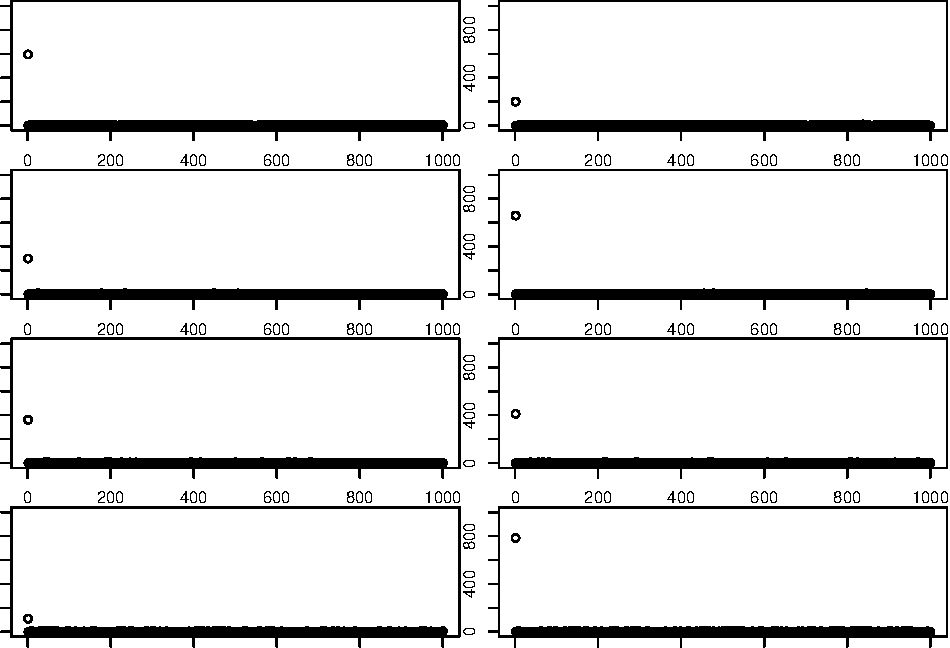
\includegraphics{./figures/unnamed-chunk-15-1.pdf}

The limiting distribution of this chain does not really depend at all on
the first value. As such initial value could be a high number (between
100-1000), given that the probability corresponding to our group number
(\(k=1\)) produces a very high \(p=\frac{1}{1+k} = \frac{1}{2}\),
therefore the chain drops very quickly to 0 and remains there without
climbing values very much.

Our maximums per simulation are always the initial value:

\begin{Shaded}
\begin{Highlighting}[]
\NormalTok{maximums }\OtherTok{=} \FunctionTok{c}\NormalTok{()}
\ControlFlowTok{for}\NormalTok{ (i }\ControlFlowTok{in} \DecValTok{1}\SpecialCharTok{:}\DecValTok{8}\NormalTok{) \{}
\NormalTok{    maximums[i] }\OtherTok{=} \FunctionTok{max}\NormalTok{(trajs[,i])}
\NormalTok{\}}
\NormalTok{maximums}
\CommentTok{\#\textgreater{} [1] 279 656 687 903 665 137 260 518}
\end{Highlighting}
\end{Shaded}

While the second highest values will be the followings:

\begin{Shaded}
\begin{Highlighting}[]
\NormalTok{maximums }\OtherTok{=} \FunctionTok{c}\NormalTok{()}
\ControlFlowTok{for}\NormalTok{ (i }\ControlFlowTok{in} \DecValTok{1}\SpecialCharTok{:}\DecValTok{8}\NormalTok{) \{}
\NormalTok{    maximums[i] }\OtherTok{=} \FunctionTok{max}\NormalTok{(trajs[,i][}\DecValTok{2}\SpecialCharTok{:}\DecValTok{1000}\NormalTok{])}
\NormalTok{\}}
\NormalTok{maximums}
\CommentTok{\#\textgreater{} [1]  8  9  8 10  9  7 10 12}
\end{Highlighting}
\end{Shaded}

Which are all significantly lower than our initial values.

\end{document}
